\documentclass{beamer}
\usepackage{lmodern}
\usepackage[labelformat=simple,
labelsep=period,
font={footnotesize},     %scriptsize, footnotesize, small, normalsize
labelfont=bf,
width=0.9\textwidth,
justification=justified,
singlelinecheck=false
]{caption}
\usepackage[utf8]{inputenc}
\usepackage[spanish, es-tabla]{babel}
\usepackage{amsmath}
\usepackage{subfigure}
\usepackage{amsfonts}
\usepackage{amssymb}
\usepackage{qtree}
\usepackage{tikz}
\usetikzlibrary{calc}
\usepackage{pgfplots,pgfplotstable}
\usepgfplotslibrary{statistics}
\usepackage[T1]{fontenc}
\usepackage{bera}
\usepackage{multirow}
\usepackage{pstricks-add}
\usepackage[capposition=top]{floatrow}
\usepackage{graphicx}
\usepackage{ragged2e}
\usepackage{float}
\usepackage[labelformat=empty]{caption}
\usepackage[justification=centering]{caption}
\setbeamersize{text margin left=5pt,text margin right=25pt}

\captionsetup[table]{labelfont={color=Brown}}
\tikzset{
	invisible/.style={opacity=0,text opacity=0}, % added text opacity to fix problems when nodes' text is opaque
	visible on/.style={alt=#1{}{invisible}},
	alt/.code args={<#1>#2#3}{%
		\alt<#1>{\pgfkeysalso{#2}}{\pgfkeysalso{#3}} % \pgfkeysalso doesn't change the path
	},
}
\pgfplotsset{compat=1.7}
    \setbeamertemplate{headline}
    {
      \leavevmode%
      \hbox{%
      \begin{beamercolorbox}[wd=.5\paperwidth,ht=2.25ex,dp=1ex,right]{section in head/foot}%
        \usebeamerfont{section in head/foot} \insertsectionhead\hspace*{2ex}
      \end{beamercolorbox}%
      \begin{beamercolorbox}[wd=.5\paperwidth,ht=2.25ex,dp=1ex,left]{subsection in head/foot}%
        \usebeamerfont{subsection in head/foot}\hspace*{2ex}\insertsubsectionhead
      \end{beamercolorbox}}%
      \vskip0pt%
    }

\setbeamertemplate{footline}
{
    \leavevmode%
    \hbox{%
        \begin{beamercolorbox}[wd=.65\paperwidth,ht=2.25ex,dp=1ex,center]{author in head/foot}%
            \usebeamerfont{author in head/foot}\insertshortauthor
        \end{beamercolorbox}%
        \begin{beamercolorbox}[wd=.05\paperwidth,ht=2.25ex,dp=1ex,center]{title in head/foot}%
            \usebeamerfont{title in head/foot}\insertshorttitle
        \end{beamercolorbox}}%
        \vskip0pt%
    }
    
    \pgfplotsset{compat=1.7}
    
    %%%%%%%%%%%%%%%%%%%%%%%%%%%%%%%%%%%%%%%%%%%%%%%%%%%%%%%%
    %%% PAra el diagrama de la diapostiva 10
    \usepackage{smartdiagram}
    \usetikzlibrary{shapes.geometric} % required in the preamble
    \smartdiagramset{
    	module minimum width=3cm,
    	module minimum height=1cm,
    	text width=4.5cm,
    	circular distance=3cm,
    }
    %%%%%%%%%%%%%%%%%%%%%%%%%%%%%%%%%%%%%%%%%%%%%%%%%%%%%%%%%%%
    \def\angle{0}
    \def\radius{2}
    \def\cyclelist{{"orange","blue","red","green"}}
    \newcount\cyclecount \cyclecount=-1
    \newcount\ind \ind=-1	
    
    
    \newcounter{saveenumi}
    \newcommand{\seti}{\setcounter{saveenumi}{\value{enumi}}}
    \newcommand{\conti}{\setcounter{enumi}{\value{saveenumi}}}
    
    \resetcounteronoverlays{saveenumi}
    \tikzset{mynode/.style={inner sep=2pt,fill,outer sep=0,circle}}

\title{Análisis Cuantitativo I}
\subtitle{Pruebas de hipótesis - Distribución t}
\author[Carlos Cardona]{Carlos Cardona Andrade}
\institute[URosario]{Universidad del Rosario}
\date{28 de octubre}


\begin{document}

\frame{\titlepage}

\begin{frame}{Quiz}
	\begin{itemize}
		\justifying
\item Un fabricante de lámparas eléctricas está ensayando un nuevo método de producción que se considerará aceptable si las lámparas obtenidas por este método dan lugar a una población normal de duración media 2400 horas, con una desviación estándar igual a 300. Se toma una muestra de 100 lámparas producidas por este método y esta muestra tiene una duración media de 2320 horas. ¿Se puede aceptar la hipótesis de validez del nuevo proceso de fabricación con un riesgo igual o menor al 5\%?
	\end{itemize}
\end{frame}

\begin{frame}{Repaso de la clase anterior}
\begin{enumerate}
\justifying
\item Se espera que una media muestra $\bar{X}$ se aproxime a la media poblacional $\mu$.
\item El error estándar provee una medida de cuán bien una media muestral se aproxima a la media poblacional.
\item Para cuantificar nuestra inferencia sobre la población, comparamos la media muestra obtenida con la media poblacional de la cual tenemos una hipótesis mediante el cálculo del z-score.
\item El objetivo de la prueba de hipótesis es determinar si la diferencia obtenida entre los datos y la hipótesis es significativamente mayor a la que esperaríamos por azar.
\end{enumerate}
\end{frame}

\begin{frame}{¿De dónde provienen los valores objetivo?}
\begin{itemize}
\justifying
\item Los valores poblaciones u objetivos de las pruebas de hipótesis pueden venir de:
\begin{enumerate}
	\justifying
\item Un parámetro poblacional conocido a partir de un grupo de comparación o de un censo poblacional (Representatividad de la muestra).
\item Parámetros conocidos a partir de un período anterior.
\item Una idea objetivo (La producción deseada en una empresa).
\end{enumerate}
\end{itemize}
\end{frame}
\begin{frame}{El problema del z-score}
	\begin{itemize}
\justifying
\item El principal inconveniente de usar el z-score para las pruebas de hipótesis es que su fórmula requiere más información de la que usualmente se tiene.
\item Específicamente, la fórmula necesita que conozcamos la desviación estándar poblacional, la cual se necesita para calcular el error estándar. 
\item La paradoja es la siguiente: se quiere utilizar el z-score para inferir información sobre una población desconocida pero, se tiene que conocer la población antes de calcularlo.
	\end{itemize}
	
\end{frame}

\begin{frame}{El error estándar estimado}
	\begin{itemize}
		\justifying
		\item Cuando se expusieron las medidas de dispersión, se explicó la diferencia de calcular la desviación estándar poblacional y la muestral.
$$s_X=\sqrt{\dfrac{\sum{(X-\bar{X})^2}}{n-1}} $$

	\item Donde $n-1$ eran los grados de libertad.
	\item Ahora para calcular el error estándar, en vez de utilizar la desviación estándar poblacional, usamos la muestral.
	$$s_{\bar{X}}=\dfrac{s_X}{\sqrt{n}}$$
	\item Cabe destacar el cambio de notación, como es un cálculo muestral, el \emph{error estándar estimado} se denota con la letra $s$ y no con $\sigma$.
		\end{itemize}
	\end{frame}
	
	\begin{frame}{El estadístico t}
\begin{itemize}
\justifying
\item El error estándar estimado se puede sustituir en la fórmula del z-score. De ahí resulta el estadístico t:
$$t=\dfrac{\bar{X}-\mu}{s_{\bar{X}}}$$
\item Este estadístico se utiliza cuando el valor de $\sigma$ es desconocido. 
\item La única diferencia entre el estadístico t y el z-score recae en el hecho que el primero utliza la desviación estándar muestral mientras que, el segundo utiliza la poblacional.
$$t=\dfrac{\bar{X}-\mu}{s_{\bar{X}}} \quad z=\dfrac{\bar{X}-\mu}{\sigma_{\bar{X}}}$$
\end{itemize}
	\end{frame}
	
	\begin{frame}{Los grados de libertad}
\begin{itemize}
\justifying
\item Se sabe que el estadístico t es un reemplazo del z-score. La diferencia básica radica en que el primero utiliza la desviación estándar muestral ($s$) mientras que, el segundo utiliza la desviación estándar poblacional ($\sigma$).
\item Para determinar qué tan bien el estadístico t se aproxima al z-score , debemos determinar qué tan bien se aproxima la desviación muestral a la poblacional.
$$s_X=\sqrt{\dfrac{\sum{(X-\bar{X})^2}}{n-1}} \quad \sigma_X=\sqrt{\dfrac{\sum{(X-\bar{X})^2}}{n}}  $$ 
\item Los grados de libertad describen el número de valores en una muestra que son independientes y libres de variar.
\end{itemize}
	\end{frame}
	
		\begin{frame}{La distribución t}
			\begin{itemize}
				\justifying
\item Toda muestra de una población puede ser utilizada para calcular tanto el z-score como el t estadístico.
\item Si se seleccionan todas las posibles muestra de tamaño $n$ y se halla el z-score para cada media muestral, entonces el conjunto de valorez z forma una distribución z.
\item De igual manera, se pueden calcular todos los estadísticos t para cada muestra y el conjunto entero de valores  t forma una distribución t.
\item Se sabe que la distribución de los z-score tiende a ser una normal si $n>30$ o las muestras provienen de una población que se distribuye normal. 
			\end{itemize}
		\end{frame}
		
\begin{frame}
\begin{itemize}
\justifying
\item Bajo esta misma situación, la distribución t se aproxima a una normal a medida que el estadístico t se aproxima a un z-score. 
\item Qué tan bien la distribución t se aproxima a una normal está determinado por los grados de libertad. En general, a media que $n$ aumenta, $n-1$ también aumenta haciendo que la distribución t se aproxime de mejor manera a la normal.
\end{itemize}
					\begin{figure}[H]
						\centering  
						\caption{} 
						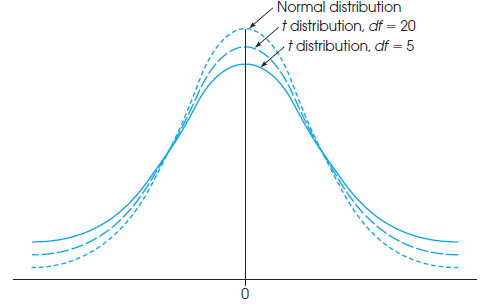
\includegraphics[width = 0.6\textwidth]{./cap2}
					\end{figure}
\end{frame}

\begin{frame}{La tabla de la distribución t}
					\begin{figure}[H]
						\centering  
						\caption{} 
						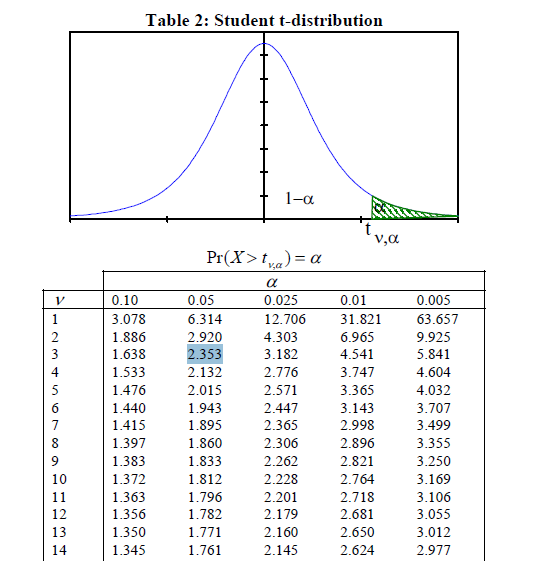
\includegraphics[width = 0.6\textwidth]{./cap1}
					\end{figure}
\end{frame}

\begin{frame}{Innate and learned perceptual abilities in the newborn infant}
	\begin{itemize}
		\justifying
		\item Los niños, incluso los recién nacidos, prefieren ver personas de caras atractivas.
		\item En esl estudio de Slater \emph{et al.}(1998), a bebés entre 1 y 6 días de nacidos se les muestra dos fotografías de mujeres. 
		\item Previamente, un grupo de adultos realiza define uno de los rostros como más atractivo que el otro. 
		\item Se ubica a los bebés enfrente de una pantalla que presenta ambos rostros durante 20 segundos.
		\item Asumamos que el estudio usa una muestra $n=9$ y obtienen una media de $\bar{X}=13$ segundos observando la cara atractiva con $s_X=3$ segundos.
	\end{itemize}
\end{frame}

\begin{frame}{Prueba de Hipótesis}
\begin{enumerate}
\justifying
\item El primer paso consiste en establecer las hipótesis y seleccionar el nivel de significancia de la prueba ($\alpha$). Aún cuando no se tiene información sobre la población, se puede definir una hipótesis lógica acerca del valor $\mu$. \\

Para este caso, la hipótesis nula afirma que no existe preferencia por ningún rostro. Por lo tanto deberían demorarse el mismo tiempo en ambos rostros.

$$H_0:\mu_{atractivo}=10$$

$$H_1:\mu_{atractivo}\neq10$$

$$\alpha=5\%$$
\seti
\end{enumerate}
\end{frame}

\begin{frame}
\begin{enumerate}
\conti
\justifying
\item El segundo paso es encontrar la región crítica. Para esto calculamos los grados de libertad:
$$n-1=9-1=8$$
Al consultar la tabla de la distribución t, con un $\alpha=$5\% encontramos que los valores críticos $t_{\alpha}=\pm2,306$
\seti
\end{enumerate}
	\begin{center}
		\scalebox{0.6}{
			\begin{tikzpicture}
			% define normal distribution function 'normaltwo'
			\def\normaltwo{\x,{4*1/exp(((\x-3)^2)/2)}}
			
			% input y parameter
			\def\x{0}
			\def\y{1}
			\def\w{5.02}
			\def\q{6}
			\def\z{3.01}
			
			
			% this line calculates f(y)
			\def\fx{4*1/exp(((\x-3)^2)/2)}
			\def\fy{4*1/exp(((\y-3)^2)/2)}
			\def\fz{4*1/exp(((\z-3)^2)/2)}
			\def\fw{4*1/exp(((\w-3)^2)/2)}
			\def\fq{4*1/exp(((\q-3)^2)/2)}
			% Shade orange area underneath curve.
			\fill [fill=orange!60] (\x,0) -- plot[domain=\x:\y] (\normaltwo) -- ({\y},0) -- cycle;
			
			\fill [fill=orange!60] (\w,0) -- plot[domain=\w:\q] (\normaltwo) -- ({\q},0) -- cycle;
			% Draw and label normal distribution function
			\draw[color=blue,domain=0:6] plot (\normaltwo) node[right] {};
			
			% Add dashed line dropping down from normal.
			\draw[dashed] ({\x},{\fx}) -- ({\x},0) node[below] {};
			\draw[dashed] ({\y},{\fy}) -- ({\y},0) node[below] {-2.306};
			\draw[dashed] ({\z},{\fz}) -- ({\z},0) node[below] {$\mu\, de \, H_0$};
			\draw[dashed] ({\w},{\fw}) -- ({\w},0) node[below] {2.306};
			\draw[dashed] ({\q},{\fq}) -- ({\q},0) node[below] {};
			% Optional: Add axis labels
			\draw (-.2,2.5) node[left] {$f_{Segundos}$};
			\draw (3,-.5) node[below] {$Segundos$};
			
			% Optional: Add axes
			\draw[->] (0,0) -- (6.2,0) node[right] {};
			\draw[->] (0,0) -- (0,5) node[above] {};
			
			\end{tikzpicture}
		}
	\end{center}
\end{frame}

\begin{frame}
\begin{enumerate}
\conti
\justifying
\item En el tercer paso se calcula el estadístico t. Para eso calculamos primero el error estándar estimado:

$$s_{\bar{X}}=\dfrac{s_X}{\sqrt{n}}=\dfrac{3}{\sqrt{9}}=\dfrac{3}{3}=1$$
Luego de esto, se halla el estadístico t:
$$t=\dfrac{\bar{X}-\mu}{s_{\bar{X}}}=\dfrac{13-10}{1}=3$$
\item El último paso consiste en tomar una decisión sobre la $H_0$. Como $t>t_{\alpha}$, nuestra decisión es rechazar la hipótesis nula y se concluye que los bebés efectivamente muestran una preferencia hacia los rostros atractivos.
\seti
\end{enumerate}
\end{frame}

\begin{frame}{Otro ejemplo}
\begin{itemize}
\justifying
\item Un dato revela que los universitarios consumen en promedio 8.8 cervezas al mes. Se toma una muestra de $n=28$ estudiantes de una universidad conservadora. Se sospecha que ahí consumen menos cervezas al mes. Probemos esta hipótesis con los siguientes datos:
$$\alpha=0.1 \quad \bar{X}=8.5 \quad s_x=1.8\, cervezas$$
\pause 
$$H_0: \mu_{muestra}\geq8.8 \quad H_1: \mu_{muestra}<8.8 $$
$$s_{\bar{X}}=\dfrac{s_X}{\sqrt{n}}=\dfrac{1.8}{\sqrt{28}}=0.34 \quad t=\dfrac{8.5-8.8}{0.34}=-0.88$$

\end{itemize}
\end{frame}

\begin{frame}
	\begin{center}
		
		\begin{tikzpicture}
		% define normal distribution function 'normaltwo'
		\def\normaltwo{\x,{4*1/exp(((\x-3)^2)/2)}}
		
		% input y parameter
		\def\x{0}
		\def\y{1.2}
		\def\w{2.5}
		\def\q{6}
		
		
		% this line calculates f(y)
		\def\fx{4*1/exp(((\x-3)^2)/2)}
		\def\fy{4*1/exp(((\y-3)^2)/2)}
		\def\fz{4*1/exp(((\z-3)^2)/2)}
		\def\fw{4*1/exp(((\w-3)^2)/2)}
		\def\fq{4*1/exp(((\q-3)^2)/2)}
		% Shade orange area underneath curve.
		\fill [fill=red!60] (\x,0) -- plot[domain=\x:\y] (\normaltwo) -- ({\y},0) -- cycle;
		
		
		
		% Draw and label normal distribution function
		\draw[color=blue,domain=0:6] plot (\normaltwo) node[right] {};
		
		% Add dashed line dropping down from normal.
		\draw[dashed] ({\x},{\fx}) -- ({\x},0) node[below] {};
		\draw[dashed] ({\y},{\fy}) -- ({\y},0) node[below] {$-1.31$};
		\draw[dashed] ({\w},{\fw}) -- ({\w},0) node[below] {$-0.88$};
		\draw[dashed] ({\q},{\fq}) -- ({\q},0) node[below] {};
		% Optional: Add axis labels
		\draw (-.2,2.5) node[left] {$f_x$};
		\draw (3,-.5) node[below] {$x$};
		
		% Optional: Add axes
		\draw[->] (0,0) -- (6.2,0) node[right] {};
		\draw[->] (0,0) -- (0,5) node[above] {};
		
		\end{tikzpicture}
	\end{center}
	$$t_{\alpha}=-1.31 \rightarrow -1.31<-0.88 \rightarrow Rechazo \quad H_0$$
\end{frame}

\begin{frame}{La representatividad de la muestra}
\begin{itemize}
\justifying
\item La representatividad de una muestra puede llevar a resultados erróneos.
\item Por ejemplo, se quiere conocer la favorabilidad de la creación de un nuevo impuesto. Para estimar esta proporción, se encuestan a personas vía telefónica.
\item Claramente, la encuesta excluye los hogares sin teléfonos, los cuales son habitados en su mayoría por personas con menores recursos.
\item Las personas con mayores ingresos son más probables de poseer la casa, por lo tanto, se ven afectados en mayor medida por el impuesto.
\end{itemize}
\end{frame}

\begin{frame}
\begin{itemize}
\justifying
\item Queremos evaluar la representatividad de la encuesta con respecto a la proporción de habitantes bajo la línea de pobreza.
\item Luego de realizar la encuesta, se identifican a 66 de las $n=387$ personas por debajo de la línea de pobreza.
\item Es decir, la proporción de personas pobre sería:
$$p_s=\dfrac{66}{387}=0.17$$
\item Además, se tiene información del censo de la población, el cual indica que el 22\% de los habitantes son pobres.
\end{itemize}
\end{frame}

\begin{frame}{La prueba de hipótesis}
\begin{itemize}
\justifying
\item Se plantean las hipótesis:
$$H_0:P_u=22\%$$

$$H_1:P_u\neq22\%$$

$$\alpha=0.05$$

$$\sigma_{Ps}=\sqrt{\dfrac{P_{u}*Q_{u}}{n}}=\sqrt{\dfrac{0.22*0.78}{387}}=0.02$$
$$t_{Ps}=\dfrac{0.17-0.22}{0.02}=\dfrac{-0.05}{0.02}=-2.5<-1.96=t_{\alpha}$$
Rechazo $H_0$ y concluyo que la muestra no es representativa.
\end{itemize}
\end{frame}



\end{document}